\documentclass[a4paper,12pt,notitlepage,pdftex,headsepline]{scrartcl}
\def\baselinestretch{1.5}
\usepackage{pdfpages}
\usepackage{cmap} % чтобы работал поиск по PDF
\usepackage[utf8x]{inputenc}
\usepackage[english,russian]{babel}
\usepackage[T2A]{fontenc}

\usepackage{textcase}
\usepackage[pdftex]{graphicx}

\pdfcompresslevel=9 % сжимать PDF
\usepackage{pdflscape} % для возможности альбомного размещения некоторых страниц
\usepackage[pdftex]{hyperref}
% настройка ссылок в оглавлении для pdf формата
\hypersetup{unicode=true,
    pdftitle={Курсовой проект по ассемблеру},
    pdfauthor={Погода Михаил},
    pdfcreator={pdflatex},
    pdfsubject={ASM},
    pdfborder    = {0 0 0},
    bookmarksopen,
    bookmarksnumbered,
    bookmarksopenlevel = 2,
    pdfkeywords={Курсовая},
    colorlinks=true, % установка цвета ссылок в оглавлении
    citecolor=black, 
    filecolor=black,
    linkcolor=black,
    urlcolor=blue
}

\usepackage{moreverb}
\author{Michael Pogoda}
\title{KursAsm}
\date{\today}

\begin{document}
\includepdf{kurstitle.pdf}
\newpage
\selectlanguage{russian}
\tableofcontents
\newpage
\addcontentsline{toc}{section}{Введение}
\large
\section*{Введение}
Применение компьютеров сейчас приобрело массовый характер.
Они используются как при научных и инженерных расчётах, хранение и обработки информации, для решении ряда других задач, так и в повседневной жизни.

Одним из основных способов вывода информации является отображение оной на мониторе.
Для того, чтобы отобразить что-либо на экране, программист должен работать некоторым образом с графическим адаптером.
Отображать информацию на мониторе можно как в графическом режиме, так и в текстовом.

Текстовые режимы были первыми, появившимися на экранах компьютеров.
В свое время даже существовали мониторы \textit{вообще} не имевшие возможности отображать графическую информацию (алфавитно-цифровые терминалы).
В применении к IBM РС-совместимым компьютерам, о текстовых режимах можно говорить как о наиболее общих для всех моделей.
Как следствие изучение их представляет достаточный интерес.

Любой вывод на экран заключается в записи пары байтов в определённое место видеопамяти.
Проделывать эту операцию в языках высокого уровня для вывода каждого символа, на наш взгляд, является неприемлимым в языках программирования высокого уровня.

Именно поэтому мы решили написать набор функций, используя которые в языках высокого уровня программист может эффективно работать с видеопамятью в текстовом режиме.
\newpage
\section{Постановка задачи}
Каждый программист сталкивается с задачей вывода информации на экран.
Иногда, работая на некоторых экзотический устройствах, программисту могут быть недоступны высокоуровневые функции вывода (которые, к слову, неявно используют низкоуровневые механизмы).

Поэтому, мы взяли на себя задачу написать модуль с функциями, который бы позволил использовать текстовый режим программистом даже в очень ,,спартанских'' условиях.
Также этот метод можно использовать с целью повышения производительности, т.\,к. зачастую вывод информации является одним из самых медленных участком программы.

Таким образом, мы должны были написать модуль, включающий в себя следующие функции:
\begin{itemize}
\item установка режима видеоадаптера;
\item считывание режима видеоадаптера;
\item считывание положения курсора;
\item установка курсора в заданную позицию;
\item вывод символа на экран в текущую позицию;
\item вывод символа на экран в заданную позицию;
\item считывание символа с экрана из текущей позиции;
\item считывание символа с экрана из заданной позиции;
\item вывод строки на экран;
\item очистка прямоугольной области экрана;
\item установка цвета фона;
\item установка цвета переднего плана;
\item установка атрибутов интенсивности и мерцания;
\item установка всех атрибутов символа;
\item считывание атрибутов символа.
\end{itemize}
\newpage
\section{Анализ существующих решений и выбор метода решения}
Все видеосистемы строятся вокруг микросхемы контроллера видео-терминала \texttt{Motorola 6845} (либо используется совместимость с этой микросхемой).
Говоря общими словами, микросхема устанавливает видеодисплей в один из нескольких алфавитноцифровых или графических режимов.
Она выполняет основную работу по интерпретации номеров кодов ASCII и поиску данных для вывода соответствующих символов в микросхеме ПЗУ (а иногда в оперативной памяти).
Она декодирует значения атрибутов цвета и соответственно устанавливает экран.
Она также создаёт курсор и управляет им.
В архитектуре EGA часть этих функций распределена между другими микросхемами.

Микросхема 6845 имеет 18 управляющих регистров, пронумерованных от 0 до 17.
Первые десять регистров фиксируют горизонтальные и вертикальные параметры дисплея.
Эти регистры, как правило, неинтересны для программистов, поскольку они автоматически устанавливаются BIOS при изменении режима экрана.
Регистры имеют размер 8 бит, но некоторые связаны в пары, чтобы хранить 16-битные величины.
Пары \#10--11 и \#14--15 устанавливают форму и местоположение курсора.
Пара \#12--13 управляет страницами дисплея.
Пара \#16--17 сообщает позицию светового пера.
Большинство регистров доступны только для чтение, только пара регистров \#14--15 доступна для записи.

Доступ ко всем 18 регистрам осуществляется через один и тот же порт, адрес которого содержится в видеопамяти по смещених \texttt{63h}.
Для записи в регистр надо сначала в регистр адреса послать номер требуемого регистра.
Тогда следующий байт, посланный в порт, с адресом на единицу больше адреса регистра адреса, будет записан в регистр.

Такой способ работы с видеопамятью называется прямым доступом к видеопамяти.
Достоинством такого способа является его быстродействие, недостатками --- отсутсвие гибкости (т.\,е. сложно написать наиболее общие функции так, чтобы они работали для всех видеорежимов) и возможность того, что в защищённом режиме прямой доступ к видеопамяти будет запрещён.

Чтобы избежать этих проблем можно использовать прерывание видео-BIOS.
Хоть они и отрабатывает немного медленнее, зато доступ к ним разрешён в защищённом режиме.

Мы выбрали основным методом использование прерывания видео-BIOS (также известному как интерфейс прерывания 10H).
Основной причиной выбора именно этого метода для нас является то, что наш модуль может быть полезен программистам, с чьим оборудованием мы формально не знакомы, но интерфейс видео-BIOS позволяет использовать те же функции для работы с текстовым режимом видеопамяти.

Более подробно с данным вопросом можно ознакомиться в \cite{wilton} и \cite{cyberguru}.
\newpage
\section{Описание выбранного решения}
Т.\,к. в постановке задачи мы чётко описали функции, которые должен реализовать наш модуль, поэтому будет логично описывать каждую функцию отдельно.

Также, т.\,к. мы широко используем прерывания, необходимо помнить процедуру выхода из программы на обработку прерывания и последующего возврата команды \texttt{INT} (см. подробнее \cite{random1}):
\begin{enumerate}
\item уменьшить указатель стека на 2 и занести в вершину стека содержимое флагового регистра;
\item очистить флаги \texttt{TF} и \texttt{IF};
\item уменьшить указатель стека на 2 и занести содержимое регистра \texttt{CS} в стек;
\item уменьшить указатель стека на 2 и занести в стек значение командного регистра;
\item обеспечить выполнение необходимых действий;
\item восстанавить из стека значение регистра и возвратить управление в прерванную программу на команду, следующую после \texttt{INT}.
\end{enumerate}
\subsection{Установка режима видеоадаптера}
Для установки видеорежима используется функция \texttt{00} прерывания \texttt{10h}.
Для её использования достаточно поместить в \texttt{AH} значение \texttt{00h} (номер функции), а в \texttt{AL} --- номер видеорежима.
Для выбора нужного видеорежима можно воспользоваться таблицей на рис.\,\ref{videomodes}.

\begin{figure}[!t]
\normalsize
\begin{tabular}{|c||c|c|c|c|c|c|}
\hline \rule[-2ex]{0pt}{5.5ex} \texttt{AL} & Тип & Формат & Цвета & Адаптер & Адрес & Монитор \\ 
\hline\hline \rule[-2ex]{0pt}{5.5ex} \texttt{0} & текст & $40\times25$ & 16/8 полутона & CGA, EGA & \texttt{B800} & Composite \\ 
\hline \rule[-2ex]{0pt}{5.5ex} \texttt{1} & текст & $40\times25$ & 16/8 & CGA, EGA & \texttt{B800} & Comp, RGB, Enhanced \\ 
\hline \rule[-2ex]{0pt}{5.5ex} \texttt{2} & текст & $80\times25$ & 16/8 полутона & CGA, EGA & \texttt{B800} & Composite \\ 
\hline \rule[-2ex]{0pt}{5.5ex} \texttt{3} & текст & $80\times25$ & 16/8 & CGA, EGA & \texttt{B800} & Comp, RGB, Enhanced \\ 
\hline \rule[-2ex]{0pt}{5.5ex} \texttt{4} & графика & $320\times200$ & 4 & CGA, EGA & \texttt{B800} & Comp, RGB, Enhanced \\ 
\hline \rule[-2ex]{0pt}{5.5ex} \texttt{5} & графика & $320\times200$ & 4 полутона & CGA, EGA & \texttt{B800} & Composite \\ 
\hline \rule[-2ex]{0pt}{5.5ex} \texttt{6} & графика & $640\times200$ & 2 & CGA, EGA & \texttt{B800} & Comp, RGB, Enhanced \\ 
\hline \rule[-2ex]{0pt}{5.5ex} \texttt{7} & текст & $80\times25$ & 3 & MA, EGA & \texttt{B000} & TTL Monochrome \\ 
\hline \rule[-2ex]{0pt}{5.5ex} \texttt{0D} & графика & $320\times200$ & 16 & EGA & \texttt{A000} & RGB, Enhanced \\ 
\hline \rule[-2ex]{0pt}{5.5ex} \texttt{0E} & графика & $640\times200$ & 16 & EGA & \texttt{A000} & RGB, Enhanced \\ 
\hline \rule[-2ex]{0pt}{5.5ex} \texttt{0F} & графика & $640\times350$ & 3 & EGA & \texttt{A000} & RGB, TTL Mono \\ 
\hline \rule[-2ex]{0pt}{5.5ex} \texttt{10} & графика & $640\times350$ & 4 или 16 & EGA & \texttt{A000} & Enhanced \\ 
\hline \rule[-2ex]{0pt}{5.5ex} \texttt{11} & графика & $640\times480$ & 2 & VGA & \texttt{A000} & RGB \\ 
\hline \rule[-2ex]{0pt}{5.5ex} \texttt{12} & графика & $640\times480$ & 16 & VGA & \texttt{A000} & RGB \\ 
\hline \rule[-2ex]{0pt}{5.5ex} \texttt{13} & графика & $640\times480$ & 256 & VGA & \texttt{A000} & RGB \\ 
\hline 
\end{tabular} 
\caption{Возможные видеорежимы}
\label{videomodes}
\end{figure}
\subsection{Считывание режима видеоадаптера}
Для того, чтобы получить номер текущего видеорежима, мы использовали функцию под номером \texttt{0F}.
Эта функция возвращает необходимое нам значение видеорежима в регистре \texttt{AL}.
\subsection{Считывание положения курсора}
Для того, чтобы определить положение курсора можно воспользовать функцией \texttt{03} прерывание видео-BIOS.
Мы решили, в качестве примера реализовать эту возможность через прямой доступ к данным видео-BIOS.

Как говорилось ранее, положение курсора хранится в паре регистров \#14--15, а т.\,к. доступ к регистрам осуществляется через регистр адреса, то вся процедура определения положения курсора сводится к следующему:
\begin{enumerate}
\item определить порт регистра адреса (он находится в видеопамяти по смещению \texttt{63h};
\item послать в этот порт 14;
\item считать из следующего за этим портом старший байт расположения курсора;
\item послать в порт регистра адреса 15;
\item считать из следующего за портом регистра адреса младший байт расположения курсора;
\item таким образом мы определили смещение курсора относительно начала видеобуффера;
\item преобразовать это значение в значения номера строки и столбца.
\end{enumerate}
Подробнее в \cite{random2} и \cite{cyberguru}.
\subsection{Установка курсора в заданную позицию}
Функция \texttt{02h} прерывания видео-BIOS позволяет установить курсор в позицию, заданную в регистрах \texttt{DH} (номер строки) и \texttt{DL} (номер столбца).
\subsection{Вывод символа на экран в текущую позицию}
Функция \texttt{0Ah} прерывания видео-BIOS выводит на экране в текущую позицию символ, указанный в \texttt{AL}, столько раз, сколько занесено в \texttt{CX}.
\subsection{Вывод символа на экран в заданную позицию}
Для того, чтобы вывести символ на экран в заданную позицию, мы используем суперпозицию функций установки положения курсора и вывода символа в текущую позицию.
\subsection{Считывание символа с экрана из текущей позиции}
Функция видео-BIOS под номером \texttt{08} позволяет считать символ из текущей позиции курсора.
После вызова прерывания, в \texttt{AH} хранятся атрибуты, а в \texttt{AL} --- символ.
\subsection{Считывание символа с экрана из заданной позиции}
Для того, чтобы считать символ с экрана из определённой позиции, достаточно просто переместить курсор в указанную позицию и считать символ, а после этого возвратиться в начальную позицию.
Это всё можно сделать, комбинирую наши предыдущие функции (считывание позиции курсора, считывание символа из текущей позиции и установка курсора в определённое позицию).
\subsection{Вывод строки на экран}
Вывод строки на экран представляет собой последовательный вывод всех символов этой строки, поэтому функция вывода строки у нас приняла вид цикла, выполняющего $n$ раз ($n$ --- длина строки) вывод очередного символа, используя прерывание видео-BIOS \texttt{0Ah}.
\subsection{Очистка прямоугольной области экрана}
Очистить прямоугольную область экрана можно используя функцию \texttt{06} прерывания \texttt{10h}, которая сдвигает экран.
Число строк, на которое нужно сдвинуть экран помещается в \texttt{AL}, и когда это число равно нулю экран очищается.
Прерывание позволяет сдвигать только часть экрана, поэтому таким образом можно очистить отдельное окно на экране.
Для этого надо поместить координаты левого верхнего угла окна в \texttt{CX}, а координаты нижнего угла в \texttt{DX} (номер строки в старший байт регистра, номер столбца --- в младший).
В \texttt{BH} необходимо занести атрибут, с которым должен чиститься экран (для этого мы узнаём атрибут в текущей позиции).
\subsection{Установка цвета фона}
Установить цвет фона можно заполнив весь экран пробелом с нужным фоном.
Тогда весь последующий текст, который будет выводится на экран, будет выводится поверх этого фона.
Мы реализовали это через вывод символа пробела с необходимым фоном 2000 раз:
в \texttt{CX} занесли 2000, в \texttt{AH} --- \texttt{09} (номер необходимой функции видео-BIOS), в \texttt{AL} --- 32 (ASCII-код символа \verb*' '), в \texttt{BL} --- атрибут цвета фона (биты 6--4 отвечают за цвет фона).
\subsection{Установка цвета переднего плана}
Установить цвет переднего плана можно аналогично с установкой цвета фона.
Необходимо знать, что биты 0--2 в регистре \texttt{BL} отвечают за цвет символа.
\subsection{Установка атрибутов интенсивности и мерцания}
Установка атрибутов интенсивности и мерцания аналогична установке цвета фона и цвета переднего плана.
В регистре \texttt{BL} бит 3 отвечает за высокую интенсивность символа, бит 7 --- за мерцание.
\subsection{Установка всех атрибутов символа}
Установка всех атрибутов является по своей сути комбинацией трёх предыдущих функций.
\subsection{Считывание атрибутов символа}
Для того, чтобы считать с экрана символ с атрибутами, достаточно вызвать функцию \texttt{08} прерывания \texttt{10h}.
Тогда в \texttt{AH} будут находится атрибуты символа.
\newpage
\section{Структура программы}
Наш проект реализован как отельный ассемблерный модуль, который содержит все описанные нами функции и константы, улучшающие читабельность кода.
Функции описаны раздельно, друг друга не вызывают.
Список функций, реализованных в модуле приведён ниже:
\begin{itemize}
\tt
\item \_SetVmode;
\item \_GetVmode;
\item \_GetCursorX;
\item \_GetCursorY;
\item \_SetCursor;
\item \_PutSymb;
\item \_PutSymbXY;
\item \_ClearRectArea;
\item \_SetBgColour;
\item \_SetTextColour;
\item \_DisplayText;
\item \_ReadChar;
\item \_ReadCharXY;
\item \_SetBlinkIntens;
\item \_SetAttr;
\item \_GetAttr.
\end{itemize}
\newpage
\section{Программная реализация}
Все функции написаны на языке assembler, следую соглашению для функций на языке C (имя функции начинается с символа подчёркивания, передача параметров происходит через стек справа налево, стек очищает вызывающая функция).
Функции, доступные из C (а также из C++ и PROLOG):
\begin{description}
\item[\texttt{void SetVmode(int n)}] устанавливает видеорежим, заданный первым параметром;
\item[\texttt{int GetVmode(void)}] возвращает текущий видеорежим;
\item[\texttt{int GetCursorX(void)}] возвращает номер столбца, в котором расположен курсор;
\item[\texttt{int GetCursorY(void)}] возвращает номер строки, в которой расположен курсор;
\item[\texttt{void SetCursor(int x, int y)}] переводит курсор в позицию, заданную параметрами (первый параметр --- номер столбца, второй --- номер строки);
\item[\texttt{void PutSymb(char a)}] выводит на экран в текущую позицию символ, заданный первым параметром;
\item[\texttt{void PutSymb(int x, int y, char a)}] выводит на экран символ, заданный третьим параметром, в позицию, заданную парой первых параметров (первый параметр характеризует номер столбца, второй --- номер строки);
\item[\texttt{void ClearRectArea(int x1, int y1, int x2, int y2)}] очищает прямоугольную область, левый верхний угол которой задан первой парой параметров, правый нижний --- второй парой;
\item[\texttt{void SetBgColour(int c)}] устанавливает цветом фона первый параметр;
\item[\texttt{void SetTextColour(int c)}] устанавливает цветов переднего плана первый параметр;
\item[\texttt{int DisplayText(char \*buf, int n)}] выводит первые n символов из строки, указатель на которую передан первым параметром, на экран в текущую позицию;
\item[\texttt{char ReadChar(void)}] возвращает символ, находящийся в текущей позиции курсора;
\item[\texttt{char ReadChar(int x, int y)}] возвращает символ, находящийся в позиции, заданной парой параметров;
\item[\texttt{void SetBlinkIntens(short blink, short intens)}] устанавливает атрибуты интенсивности и мерцания в соотвествии с параметрами (первый параметр отвечает за мерцание, второй --- за интенсивность);
\item[\texttt{void SetAttr(short blink, short bgcol, short intens, short col)}] устанавливает все атрибуты текста (первый параметр отвечает за мерцание, второй --- за цвет фона, третий --- за мерцание, четвёртый --- за цвет переднего плана);
\item[\texttt{short GetAttr(void)}] возвращает все атрибуты символа (биты 0--2 отвечают за цвет переднего плана, бит 3 --- за интенсивность, биты 4--6 --- за цвет фона, бит 7 --- за мерцание).
\end{description}
\newpage
\section{Руководство пользователя}
\subsection*{Системные требования}
\begin{itemize}
\item IBM PC совместимый ПК;
\item Видеоадаптер, совместимый с Motorola 6845 (например, EGA или VGA);
\item Операционная системы DOS.
\end{itemize}
Чтобы использовать функции из нашего модуля для работы с видеопамятью в текстовом режиме, программист должен подключить заголовочный файл, содержащий прототипы функций на языке программирования C.
После этого можно обращаться к функциям, объявленным в заголовочном файле (перечислены в предыдущем разделе).
Для того, чтобы функции работали необходимо компилировать исходный файл на языке высокого уровня вместе с нашим ассемблерным модулем.
\newpage
\addcontentsline{toc}{section}{Заключение}
\section*{Заключение}
Написанный нами модуль позволяет программисту работать с видеопамятью в текстовом режиме из языков высокого уровня (C, C++, PROLOG).
Все функции будут работать на персональном компьютере, удовлетворяющем системным требованиям, что включает в себя широкий спетр моделей.
Среди достоинств нашего модуля стоит отметить, что программист может использовать его как в реальном, так и в защищённом режимах.
Среди недостатков можно отметить то, что функции, реализованные в модуле, медленнее своих аналогов, заточенных под конкретные режимы и работающие в реальном режиме.
\newpage
\addcontentsline{toc}{section}{Литература}
\begin{thebibliography}{0}
\bibitem{wilton}
Уилтон Р. Видиосистемы персональных компьютеров IBM PC и PS/2. Руководство по программированию: Пер. с англ. К.\,Г. Смирнова; Под ред. В.\,Л. Григорьева. --- М.:Радио и связь, 1994. --- 384 с.:ил.
\bibitem{random1}
Фельдман С.\,К. Системное программирование на персональном компьютере. 2е изд. --- М.: Бук пресс, 2006. --- 512 с.
\bibitem{random2}
\url{http://vx.netlux.org/lib/files/vik00\_ru/boot.asm}
\bibitem{cyberguru}
\url{http://www.cyberguru.ru/programming/assembler/programming-video-output.html}
\end{thebibliography}
\newpage
\addcontentsline{toc}{section}{Приложения}
\def\baselinestretch{1}
\section*{Приложения}
\subsection*{Приложение A}
\subsubsection*{module.asm}
\begin{footnotesize}

\listinginput{1}{module.asm}\end{footnotesize}

\newpage
\subsection*{Приложение B}
\begin{figure}[!h]
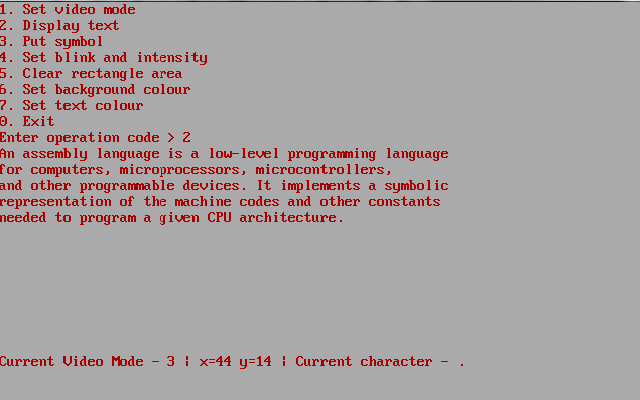
\includegraphics[scale=1]{1.png}
\caption{Пример использования модуля}
\end{figure}
%\bibliography{kurs2}
\end{document}
